\documentclass[tikz,border=8pt]{standalone}
% Shared look for every TikZ diagram. Load with % Shared look for every TikZ diagram. Load with % Shared look for every TikZ diagram. Load with \input{../../tools/tikz-style.tex}
\usepackage[T1]{fontenc}
\usepackage{lmodern}
\renewcommand{\sfdefault}{lmr}  % diagrams use the same serif as the text
\usetikzlibrary{arrows.meta, positioning, shapes.geometric, calc, fit, backgrounds}
\definecolor{cblue}{HTML}{4C78A8}
\definecolor{corange}{HTML}{F58518}
\definecolor{cgreen}{HTML}{54A24B}
\definecolor{cred}{HTML}{E45756}
\definecolor{cpurple}{HTML}{B279A2}
\definecolor{cgrey}{HTML}{6B6B6B}
\tikzset{
  every picture/.style={font=\sffamily, line width=1.2pt},
  box/.style={draw=#1, fill=#1!12, rounded corners=4pt, align=center, inner sep=7pt, minimum height=1.1cm},
  box/.default=cgrey,
  arrow/.style={-{Stealth[length=3mm]}, draw=cgrey, line width=1.4pt},
  title/.style={font=\sffamily\bfseries\Large},
  note/.style={font=\sffamily\small, text=cgrey, align=center},
}
\AtBeginDocument{\hyphenpenalty=10000 \exhyphenpenalty=10000}

\usepackage[T1]{fontenc}
\usepackage{lmodern}
\renewcommand{\sfdefault}{lmr}  % diagrams use the same serif as the text
\usetikzlibrary{arrows.meta, positioning, shapes.geometric, calc, fit, backgrounds}
\definecolor{cblue}{HTML}{4C78A8}
\definecolor{corange}{HTML}{F58518}
\definecolor{cgreen}{HTML}{54A24B}
\definecolor{cred}{HTML}{E45756}
\definecolor{cpurple}{HTML}{B279A2}
\definecolor{cgrey}{HTML}{6B6B6B}
\tikzset{
  every picture/.style={font=\sffamily, line width=1.2pt},
  box/.style={draw=#1, fill=#1!12, rounded corners=4pt, align=center, inner sep=7pt, minimum height=1.1cm},
  box/.default=cgrey,
  arrow/.style={-{Stealth[length=3mm]}, draw=cgrey, line width=1.4pt},
  title/.style={font=\sffamily\bfseries\Large},
  note/.style={font=\sffamily\small, text=cgrey, align=center},
}
\AtBeginDocument{\hyphenpenalty=10000 \exhyphenpenalty=10000}

\usepackage[T1]{fontenc}
\usepackage{lmodern}
\renewcommand{\sfdefault}{lmr}  % diagrams use the same serif as the text
\usetikzlibrary{arrows.meta, positioning, shapes.geometric, calc, fit, backgrounds}
\definecolor{cblue}{HTML}{4C78A8}
\definecolor{corange}{HTML}{F58518}
\definecolor{cgreen}{HTML}{54A24B}
\definecolor{cred}{HTML}{E45756}
\definecolor{cpurple}{HTML}{B279A2}
\definecolor{cgrey}{HTML}{6B6B6B}
\tikzset{
  every picture/.style={font=\sffamily, line width=1.2pt},
  box/.style={draw=#1, fill=#1!12, rounded corners=4pt, align=center, inner sep=7pt, minimum height=1.1cm},
  box/.default=cgrey,
  arrow/.style={-{Stealth[length=3mm]}, draw=cgrey, line width=1.4pt},
  title/.style={font=\sffamily\bfseries\Large},
  note/.style={font=\sffamily\small, text=cgrey, align=center},
}
\AtBeginDocument{\hyphenpenalty=10000 \exhyphenpenalty=10000}

\begin{document}
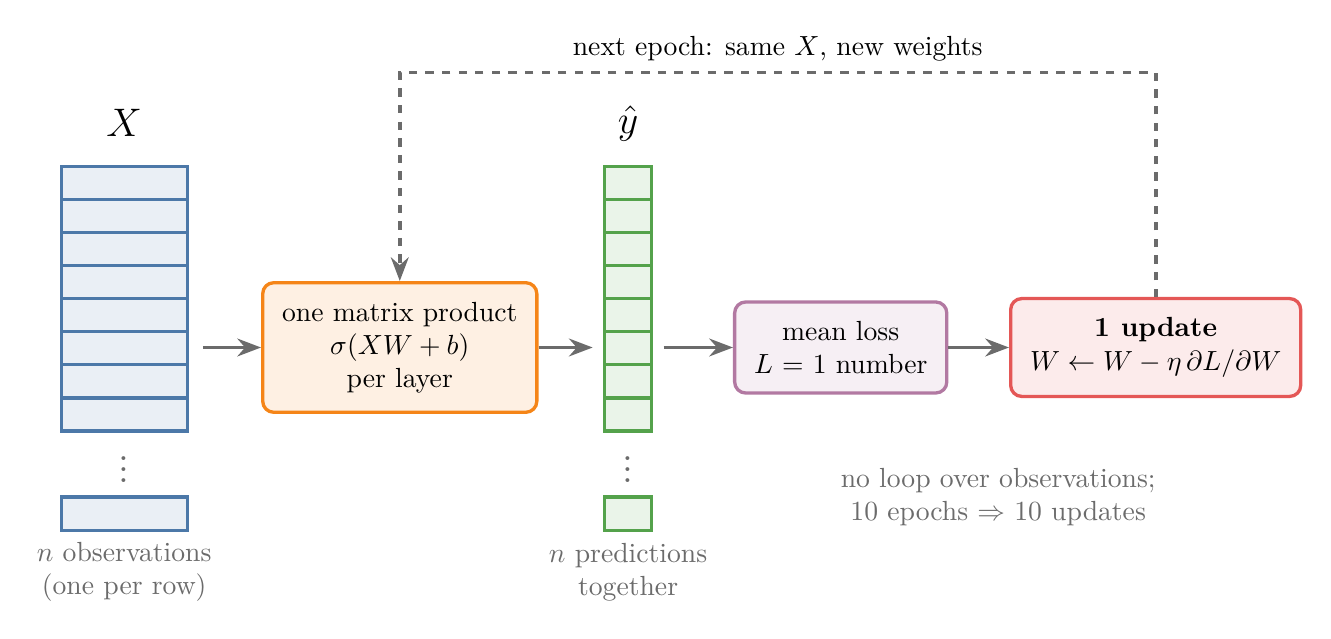
\begin{tikzpicture}
  % X: n rows stacked as one matrix
  \foreach \i in {0,...,7} \draw[cblue, fill=cblue!12] (0,-0.42*\i) rectangle (1.6,-0.42*\i-0.42);
  \node[cgrey] at (0.8,-3.75) {\Large$\vdots$};
  \draw[cblue, fill=cblue!12] (0,-4.2) rectangle (1.6,-4.62);
  \node[title] at (0.8,0.55) {$X$};
  \node[note, font=\sffamily\normalsize] at (0.8,-5.15) {$n$ observations\\(one per row)};
  % one matrix product
  \node[box=corange, minimum width=3.2cm] (mp) at (4.3,-2.3) {one matrix product\\$\sigma(XW+b)$\\per layer};
  \draw[arrow] (1.8,-2.3) -- (mp.west);
  % n predictions
  \foreach \i in {0,...,7} \draw[cgreen, fill=cgreen!12] (6.9,-0.42*\i) rectangle (7.5,-0.42*\i-0.42);
  \node[cgrey] at (7.2,-3.75) {\Large$\vdots$};
  \draw[cgreen, fill=cgreen!12] (6.9,-4.2) rectangle (7.5,-4.62);
  \node[title] at (7.2,0.55) {$\hat y$};
  \node[note, font=\sffamily\normalsize] at (7.2,-5.15) {$n$ predictions\\together};
  \draw[arrow] (mp.east) -- (6.75,-2.3);
  % mean loss, one update
  \node[box=cpurple] (L) at (9.9,-2.3) {mean loss\\$L$ = 1 number};
  \draw[arrow] (7.65,-2.3) -- (L.west);
  \node[box=cred] (U) at (13.9,-2.3) {\textbf{1 update}\\$W \leftarrow W-\eta\,\partial L/\partial W$};
  \draw[arrow] (L.east) -- (U.west);
  \draw[arrow, dashed] (U.north) -- ++(0,2.85) -| node[pos=0.25, above, font=\sffamily\normalsize] {next epoch: same $X$, new weights} (mp.north);
  \node[note, font=\sffamily\normalsize] at (11.9,-4.2) {no loop over observations;\\10 epochs $\Rightarrow$ 10 updates};
\end{tikzpicture}
\end{document}
